\documentclass{article}
\usepackage[utf8]{inputenc}
\usepackage[spanish]{babel}
\usepackage{listings}
\usepackage{graphicx}
\graphicspath{ {images/} }
\usepackage{cite}

\begin{document}

\begin{titlepage}
    \begin{center}
        \vspace*{1cm}
            
        \Huge
        \textbf{Memoria del computador y su funcionamiento}
            
        \vspace{0.5cm}
        \LARGE
        Informática 2
            
        \vspace{1.5cm}
            
        \textbf{Mateo Ricaurte}
            
        \vfill
            
        \vspace{0.8cm}
            
        \Large
        Despartamento de Ingeniería Electrónica y Telecomunicaciones\\
        Universidad de Antioquia\\
        Medellín\\
        Septiembre de 2020
            
    \end{center}
\end{titlepage}

\tableofcontents
\newpage
\section{Introducción}
Vamos a responder algunas preguntas del texto del profesor Augusto acerca de la memoria del computador, el manejo y procedimiento que se utiliza para así saber un poco más sobre como funciona un ordenador, de manera eficiente y rápida respecto a la información que se en encuentra en el ordenador.
\newpage
\section{Respuestas del cuestionario} \label{contenido}
\subsection{Defina que es la memoria del computador.}

La memoria es un sistema donde se almacena cierta información de manera temporal que algún usuario requiere en ese instante para hacer alguna tarea o alguna orden en el computador cierta información la puede recibir la memoria gracias a microprocesadores que viajan del disco duro hacia la memoria a través de un canal o como se dice técnicamente bus de datos. Este procedimiento se repite varias veces, las necesarias para que los datos cambien, se procesen o se modifiquen y así se haga de manera correcta.
\paragraph{}
La memoria en un computador hace que el funcionamiento de este sea eficiente gracias a que existen diferentes tipos de memoria que se encargan de guardar datos e información de cada aplicación del computador. Sin embargo, por más de que el disco duro y la memoria son dos dispositivos de almacenamiento del computador, la memoria tiene mayor velocidad y esto hace que el procedimiento de buscar la información que deseemos en cierto momento sea en cuestión de instantes y de manera eficiente, si este procedimiento se hiciera en un disco duro, todo sería mucho más lento y el usuario debería esperar más tiempo para obtener lo que desee. De las partes que conforman el procedimiento de obtención de información como lo es la memoria, el disco duro, los microprocesadores, los buses de datos; la memoria es la parte más importante de este proceso mientras el computador esté encendido.

\paragraph{}
A continuación se presenta el funcionamiento de datos en una computadora Figura. (\ref{fig:imagen1})
\paragraph{}

\begin{figure}[h]
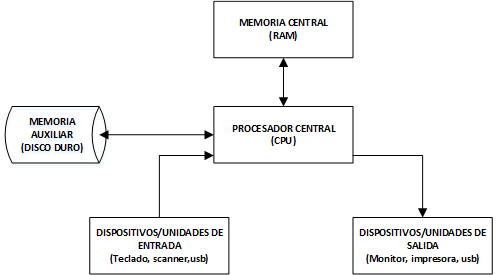
\includegraphics[width=10cm]{imagen1.png}
\centering
\caption{Arquitectura de Von Neumman \cite{img1}}
\label{fig:imagen1}
\end{figure}
\subsection{Mencione los tipos de memoria que conoce y haga una pequeña descripción de cada tipo.}
\paragraph{}
\subsubsection{Memoria Cache.}	
Es la memoria que mayor velocidad tiene, aunque su almacenamiento no es muy grande, ya que esta memoria es muy costosa y no podría ocupar mayor espacio en un computador de rama comercial. Esta memoria tiene una pequeña parte de la memoria principal (memoria RAM). Cada vez que el computador necesite saber algo como por ejemplo leer una palabra, esta debe pasar por la comprobación mediante la memoria cache.
\paragraph{}
Como apreciamos en el texto\cite{texto} la memoria cache tiene 3 niveles:
\paragraph{}
•	L1: Tiene una capacidad de almacenar instrucciones de 32 kb, es la más rápida de los 3 niveles y se encuentra ubicada en el núcleo del microprocesador.
\paragraph{}
•	L2: Tiene una capacidad de almacenamiento de 256 kb, tiene mayor capacidad que L1, pero es un poco más lenta.
\paragraph{}
•	L3: Es la que mas lento corre de los 3 niveles, su capacidad de almacenamiento es de 12 Mb, se encuentra ubicado dentro del procesador, pero no dentro de su núcleo. 
\begin{figure}[h]
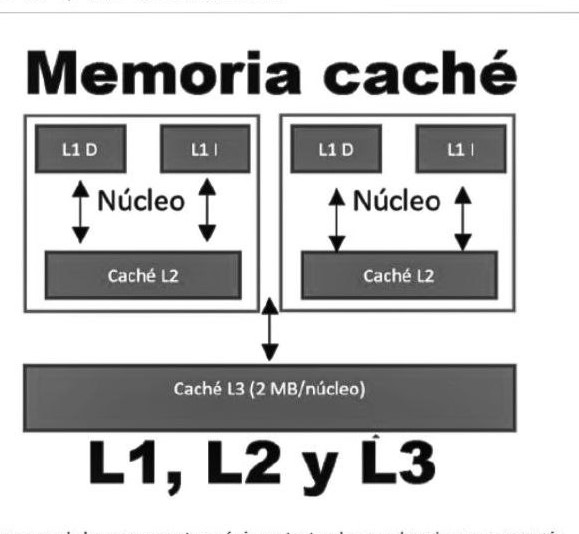
\includegraphics[width=8cm]{imagen2.jpg}
\centering
\caption{Memoria Caché. \cite{img2}}
\label{fig:imagen2}
\end{figure}
\paragraph{}

\subsubsection{Memoria RAM (Random Access Memory-Memoria de Acceso Aleatorio).}


Es la memoria principal del ordenador, corre más lento que la memoria cache pero esta memoria se la puede conseguir a un precio más accesible y comercial. La mayoría de las instrucciones que el usuario le ordena al computador se encuentran en esta memoria en el momento en que se las pida. Esta memoria es dividida por celdas donde se encuentran ubicados todos lo bits representados por varios unos y ceros, los cuales llevan la información y son trabajados por el microprocesador.

\begin{figure}[h]
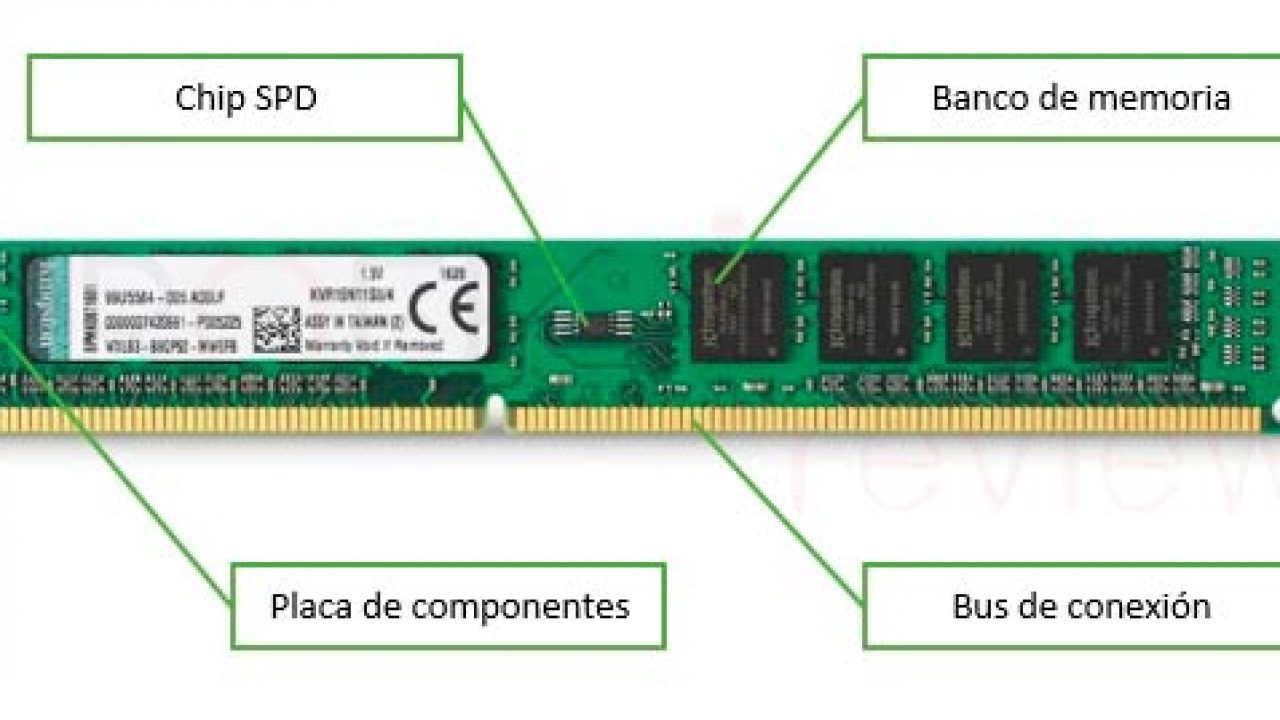
\includegraphics[width=10cm]{imagen3.jpg}
\centering
\caption{Memoria RAM. \cite{img3}}
\label{fig:imagen3}
\end{figure}
\paragraph{}
\subsubsection{Memoria virtual.}

Es una pequeña parte de la memoria del disco duro y su principal función es ayudar de manera remota a almacenar pequeñas porciones de los programas, así como también algunos datos que innecesariamente están ejecutándose en ese momento. Esta memoria nos sirve para despejar un poco de almacenamiento a la memoria RAM que no es necesaria y se la montamos a esta memoria y esto hará que el espacio liberado en la memoria RAM sea utilizado por otros recursos más primordiales.

\begin{figure}[h]
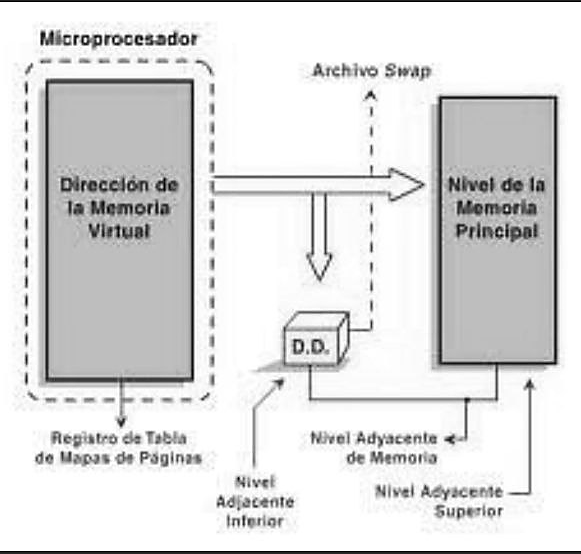
\includegraphics[width=6cm]{imagen4.png}
\centering
\caption{proceso de funcionamiento de la memoria virtual\cite{img4}.}
\label{fig:imagen4}
\end{figure}
\paragraph{}
\subsubsection{Disco Duro.}
En esta memoria es donde se ubica toda la información que tiene el computador y es de donde la memoria abstrae los datos que el usuario quiere que vayan a ser modificados. Su procedimiento se hace de manera magnética. En el disco duro se encuentra guardado toda la información del computador y se guarda de manera permanente todos sus datos, esto hace que la información no se borre ni siquiera cuando la computadora está apagada. Es de aquí de donde se puede enviar la información a los distintos tipos de almacenamiento para que realicen su trabajo y hagan que el sistema de almacenamiento funcione.
\\
\begin{figure}[h]
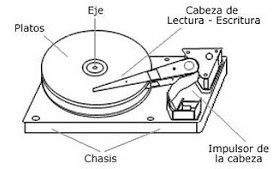
\includegraphics[width=8cm]{imagen5.jpg}
\centering
\caption{Disco Duro\cite{img5}.}
\label{fig:imagen5}
\end{figure}
\newpage
\subsection{Describa la manera como se gestiona la memoria en un computador.}
\paragraph{}
La memoria del computador es gestionada gracias al sistema operativo el cual hace que funcione el procedimiento de traspaso de información, de un tipo de almacenamiento hacia el otro. Mientras este procedimiento se está ejecutando, a su vez, se está comprobando el espacio de almacenamiento que se tiene en cada tipo de memoria, para que así se lleve un registro de actividad y haga que el computador funcione de manera eficiente, así como lo dice Enrico Sagnotti en su escrito\cite{memoria}. Todo archivo que acceda el usuario en el computador se carga primero a la memoria RAM con el fin de que se logre obtener la información de manera rápida y así este proceso (que por cierto se hace demasiadas veces por segundo mientras está funcionando el computador), evite que el sistema operativo colapse o deje de funcionar. Este proceso funciona de manera correcta al abrir algo que el usuario desea y en el momento en que ya no queremos esa información, simplemente la cerramos y esto hará que automáticamente se quiten de manera instantánea de la memoria del computador, pero hay que tener precaución sobre si queremos que nuestras modificaciones en el archivo que estamos utilizando las guardemos en el disco duro, si no hacemos esto, se perdería cierta información de manera permanente.

\paragraph{}
\subsection{¿Qué hace que una memoria sea más rápida que otra? ¿Por qué esto es importante?.}
4.	La diferencia de velocidades entre las memorias que tiene el computador es por el tiempo que tarda el bus de datos en procesar la información y pasa por la placa madre la cual hace que se lleven los datos de un lugar a otro, añadido de un tiempo que tarda el bus de datos enlazando con el microprocesador toda la información que se le solicite al computador. Es por eso por lo que existe cierta jerarquía en las memorias, siendo la memoria cache la mas veloz, seguida de la memoria RAM, luego está la memoria virtual y por último el disco duro, así como dice en el texto de Augusto \cite{documento}. En cada memoria existe cierta latencia que hace que las memorias tengan fallos de velocidad y haga que una se demore más que la otra con el fin de medir su eficiencia.

Es importante la velocidad de las memorias ya que sabiendo esto podemos clasificar los tipos de información para asignarle a cada tipo de memoria, es por la velocidad de las memorias que algunas tienen mas costo que otras, pero hay que tener en cuenta que todas las memorias van unidas en este proceso para que así el sistema operativo del ordenador funcione de manera correcta. 
\newpage
\section{Conclusión} \label{conclusion}
Existen muchos tipos de memorias que ayudan a que el computador mejore cada vez más, cada tipo de memoria tiene diferentes funciones que cumplir y datos distintos los cuales ejecutar en cierto momento que se lo requiera, la memoria es un factor muy importante en el computador para que logre funcionar de manera precisa y correcta.
\newpage
\bibliographystyle{IEEEtran}
\bibliography{references}

\end{document}
